\section{El paso de un espacio de coordenadas a otro.}
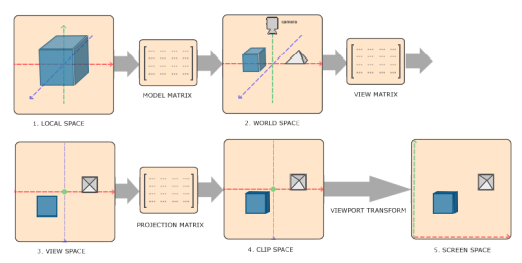
\includegraphics{space_coordinates_process.png}

Como se ve, la mayor parte de las transformaciones están hechas con matrices.
Específicamente hay tres: la \emph{matriz de modelado}, la \emph{matriz de visión} y la \emph{matriz de proyección}.

La \emph{matriz de modelado} puede traducir, escalar o rotar al objeto para moverlo de su localización inicial, modificar su tamaño o cambiar su orientación. Es decir, convierte las coordenadas locales a globales.

La \emph{matriz de visión} es la que se encarga de transformar los objetos a través de traducciones y rotaciones para traducir/rotar la escena para que se vean frente a la cámara. Estas transformaciones se le hacen a las coordenadas obtenidas en el espacio global.

Y la \emph{matriz de proyección} permite que se utilicen rangos de coordenadas como $[-3000, 3000]$ en cada eje y se le pasen así a la shader de vértices para luego normalizarlas a un rango $[-1.0, 1.0]$ que acepta OpenGL. Así todos los vértices que tengan una coordenada menor a -1.0 o mayor a 1.0 son recortados. Se ve que la matríz de proyección crea una "caja de visualización" a la que se llama \emph{frustum} en inglés, las coordenas que queden dentro del \emph{frustum} se verán en pantalla. Además, esta matriz puede ser una matriz de proyección \emph{ortográfica} o \emph{de perspectiva}.

Hay que destacar que luego de que los vértices estén en el espacio de recorte, se lleva a cabo la \emph{división de perspectiva} en la que se convierten el espacio de recorte 4D a NDC 3D. Esto se hace dividiendo las componentes $x, y, z$ entre la componente $w$.

Por último, se da la transformación de ventana gráfica (viewport), etapa en la que se mapean las NDC a los valores específicados por \lstinline{glViewport}.

\subsection{Proyección ortográfica.}
En esta se define un frustum cúbico que define el espacio de recortado donde cualquier vértice fuera de esta caja no se muestra. Se ve así:

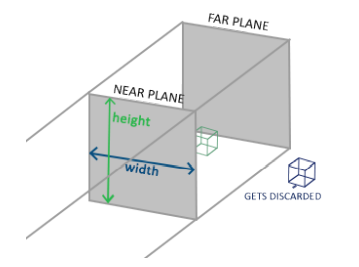
\includegraphics{ortographic_proy.png}

Lo que esté fuera del ancho, largo o esté más allá del plano lejano se recortará. Este método mapea las coordeanadas dentro del frustum a NDC sin efectos secundarios (por ejemplo, no toma en cuenta la perspectiva por lo que se pueden obtener resultados extraños) ya que no usa la componente $w$; si esta última es 0 la división de perspectiva no tiene efecto. Así se crea una matriz de proyección ortográfica con GLM:

\begin{lstlisting}
    glm::ortho(x1, x2, y1, y2, z1, z2);
\end{lstlisting}

Donde el rango x1 a x2 es el ancho, el de y1 a y2 el alto y el de z1 a z2 la distancia entre el plano cercano y el lejano.

\subsection{Proyección de perspectiva.}
Esta proyección hace que lo que esté más cerca del observador se vea más grande que lo que está lejos. La matrix de proyección de perspectiva mapea un rango de frustum dado al espacio de recortado (donde todas las coordenadas están entre -1.0 y 1.0) y manipula la componente $w$ para que se haga más grande entre más lejos el vértice. Luego de que se esté en el espacio de recorte, se hace la divisón de perspectiva en las coordenadas así:

\begin{center}
\begin{equation*}
out = \left(\begin{array}{c}
      x/w \\
      y/w \\
      z/w \\
      \end{array}\right)
\end{equation*}
\end{center}

Para crear una matriz de proyección de perspectiva en GLM se hace así:

\begin{lstlisting}
    glm::mat4 proj = glm::perspective(fov, 
                                     relacion de aspecto, 
                                     z1, z2);
\end{lstlisting}

Donde \lstinline{fov} está en radianes con \lstinline{glm::radians(grados)}, \lstinline{relacion de aspecto} es $anchura / altura$ (ambos parámetros 
de la ventana gráfica) y z1 y z2 la distancia hasta 
el plano cercano (usualmente 0.1) y hasta el plano lejano respectivamente.

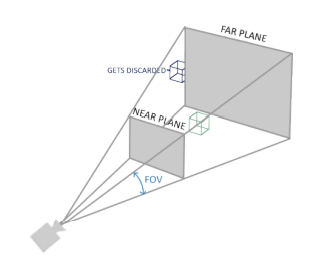
\includegraphics{perspective_proy.png}